\documentclass[letterpaper,10pt]{amsart}

\usepackage[pdftex]{graphicx}
\usepackage{moreverb}
\usepackage{amsmath}
\usepackage{amsthm}
\usepackage{fullpage}
\usepackage{amssymb}
\usepackage{tikz}
\usepackage{dsfont}
\usepackage{hyperref}
\usepackage[all]{xy}
\usepackage{bbm}
\usepackage{mathtools}
\usepackage[margin=0.5in]{geometry}
\usepackage{enumerate}
\usepackage{multirow}
\usepackage{cancel}


\newcommand{\sumin}{\sum_{i=1}^n}
\newcommand{\sumjn}{\sum_{j=1}^n}
\newcommand{\sumiN}{\sum_{i=1}^N}
\newcommand{\sumjN}{\sum_{j=1}^N}
\newcommand{\sumim}{\sum_{i=1}^m}
\newcommand{\sumjm}{\sum_{j=1}^m}
\newcommand{\prodin}{\prod_{i=1}^n}
\newcommand{\rmd}{\mathrm{d}}
\newcommand{\dx}{\,\mathrm{d}x}
\newcommand{\dy}{\,\mathrm{d}y}
\newcommand{\dt}{\,\mathrm{d}t}
\newcommand{\dz}{\,\mathrm{d}z}
\newcommand{\dmu}{\,\mathrm{d}\mu}
\newcommand{\dnu}{\,\mathrm{d}\nu}
\newcommand{\dP}{\,\mathrm{d}\mathbb{P}}
\newcommand{\fa}{\; \forall \;}


%distributions and functions
\newcommand{\E}[1]{\mathbb{E}\!\left[#1\right]}
\newcommand{\Esub}[2]{\mathbb{E}_{#1}\left[#2\right]}
\newcommand{\p}[1]{\mathbb{P}\!\left(#1\right)}
\newcommand{\psub}[2]{\mathbb{P}_{#1}\left(#2\right)}
\newcommand{\tr}{\operatorname{tr}}
\newcommand{\Var}{\operatorname{Var}}
\newcommand{\Cov}{\operatorname{Cov}}
\newcommand{\Corr}{\operatorname{Corr}}
\newcommand{\argmax}{\operatorname*{arg \, max}}
\newcommand{\argmin}{\operatorname*{arg \, min}}
\newcommand{\Beta}{\textnormal{Beta}}
\newcommand{\Bin}{\textnormal{Bin}}
\newcommand{\logit}{\operatorname{logit}}
\newcommand{\Gammadist}{\textnormal{Gamma}}
\newcommand{\Geom}{\textnormal{Geom}}
\newcommand{\Expo}{\textnormal{Expo}}
\newcommand{\Pois}{\textnormal{Pois}}
\newcommand{\Unif}{\textnormal{Uniform}}
\newcommand{\Bern}{\textnormal{Bern}}
\newcommand{\sgn}{\operatorname{sgn}}
\newcommand{\Mult}{\textnormal{Mult}}
\newcommand{\MVN}{\textnormal{MVN}}


%special letters
\newcommand{\sA}{\mathcal{A}}
\newcommand{\sB}{\mathfrak{B}}
\newcommand{\sC}{\mathcal{C}}
\newcommand{\sD}{\mathcal{D}}
\newcommand{\sF}{\mathcal{F}}
\newcommand{\sG}{\mathcal{G}}
\newcommand{\sH}{\mathcal{H}}
\newcommand{\sI}{\mathcal{I}}
\newcommand{\sL}{\mathcal{L}}
\newcommand{\sP}{\mathcal{P}}
\newcommand{\sQ}{\mathbb{Q}}
\newcommand{\sR}{\mathbb{R}}
\newcommand{\sS}{\mathcal{S}}
\newcommand{\sT}{\mathcal{T}}
\newcommand{\sX}{\mathcal{X}}
\newcommand{\indep}{\perp\!\!\!\perp}
\newcommand{\io}{\text{ i.o.}}

\newtheorem*{prop}{Prop}
\newtheorem{theorem}{Theorem}
\newtheorem*{claim}{Claim}
\newtheorem*{corollary}{Corollary}
\newtheorem{defn}{Definition}
\newtheorem{ex}{Example}
\newtheorem*{lemma}{Lemma}
\newtheorem*{exercise}{Exercise}

\newenvironment{verbatimcode}{\bigskip \scriptsize \verbatim}{\endverbatim \normalsize \bigskip}
\allowdisplaybreaks

\begin{document}

\title{STAT 221 - Assignment 4}
\author{Greg Tam, Student ID: 70908239}
\date{}
\maketitle


\begin{enumerate}[{1}.1]
\item First, we reparameterize $\mu$ as $\lambda = \theta \cdot \mu$ so that
\begin{align*}
\E{Y_i | \theta, \mu} &= \E{\E{Y_i | \theta, \mu, N}}\\
&= \E{N \theta}\\
&= \theta \cdot \mu\\
&= \lambda
\end{align*}
The suggested distribution we are given is $\p{\lambda, \theta} \propto \lambda^{-1}$. We do a change of variables from $(\lambda, \theta)$ to $(\mu, \theta)$. Define $g_1, g_2$ as
\begin{align*}
g_1(\lambda, \theta) &= \frac{\lambda}{\theta} = \mu\\
g_2(\lambda, \theta) &= \theta
\end{align*}
and their inverses, $h_1, h_2$, are
\begin{align*}
h_1(\mu, \theta) &= \theta \cdot \mu = \lambda\\
h_2(\mu, \theta) &= \theta
\end{align*}
respectively. Now, this gives us our Jacobian for the transformation
\[|J| = \begin{vmatrix}
\frac{\partial h_1}{\partial \mu} & \frac{\partial h_1}{\partial \theta}\\
\frac{\partial h_2}{\partial \mu} & \frac{\partial h_2}{\partial \theta}
\end{vmatrix} = \begin{vmatrix}
\theta & \mu\\
0 & 1
\end{vmatrix} = \theta \]
So our prior distribution on $(\mu, \theta)$ is
\begin{align*}
\p{\mu, \theta} &= \p{h_1(\mu, \theta), h_2(\mu, \theta)} |J|\\
&= \p{\mu \theta, \theta} \theta\\
&= \frac{1}{\mu \theta} \theta \mathds{1}_{\theta \in [0,1]} \\
&\propto \frac{1}{\mu} \mathds{1}_{\theta \in [0,1]}
\end{align*}
Using this, we have that
\begin{align*}
\p{N, \theta} &= \int \! \p{N, \theta, \mu} \, \rmd \mu \\
&= \int_0^\infty \! \p{N | \theta, \mu} \p{\mu, \theta} \, \rmd \mu \\
&\propto \int \! \frac{\mu^N}{N!}e^{-\mu} \frac{1}{\mu}  \mathds{1}_{\theta \in [0,1]} \, \rmd \mu\\
&= \frac{1}{N!} \mathds{1}_{\theta \in [0,1]} \int_0^\infty \! \mu^{N-1} e^{-\mu} \, \rmd \mu\\
&= \frac{\Gamma(N)}{N!} \mathds{1}_{\theta \in [0,1]}\\
&= \frac{1}{N} \mathds{1}_{\theta \in [0,1]}
\end{align*}
This is sensible as the probability of sampling $N$ is less likely the larger $N$ is and more likely the smaller $N$ is. 

\item The support of $\lambda$ is $(0,\infty)$ and the support of $\theta$ is $[0,1]$. If we take
\begin{align*}
\int_0^\infty \int_0^1 \! \p{\lambda, \theta} \, \rmd \theta \rmd \lambda &= \int_0^\infty \int_0^1 \! \frac{1}{\lambda} \, \rmd \theta \rmd \lambda\\ 
&= \infty
\end{align*}
and because this is finite, we cannot get a normalizing constant, so this prior is not proper.


\item
We have that $Y_1, \ldots, Y_n \sim \Bin(N, \theta)$, so that
\[\p{Y_i = y_i | N, \theta} = \binom{N}{y_i} \theta^N (1-\theta)^{N - y_i}\]
To get $\p{Y_i | \mu, \theta}$, we take
\begin{align*}
\p{Y_i = y_i | \mu, \theta} &= \sum_{n=y_i}^\infty \p{Y_i = y_i, N=n | \mu, \theta}\\
&= \sum_{n=y_i}^\infty \p{Y_i = y_i | N=n, \mu, \theta} \p{N=n | \mu, \theta}\\
&= \sum_{n=y_i}^\infty \p{Y_i = y_i | N=n, \theta} \p{N=n | \mu, \theta}\\
&= \sum_{n=y_i}^\infty \binom{n}{y_i}\theta^{y_i} (1-\theta)^{n-y_i} \frac{\mu^n}{n!}e^{-\mu}\\
&= \sum_{n=y_i}^\infty \frac{1}{y_I! (n - y_i)!} \theta^{y_i} (1-\theta)^{n - y_i} \mu^n e^{-\mu}\\
&= \frac{(\theta \mu)^{y_i} e^{-\mu}}{y_i!} \sum_{n = y_i}^\infty \frac{(1-\theta)^{n-y_i}}{(n-y_i)!}\mu^{n-y_i}
\end{align*}
Now, reparameterizing this buy letting $t = n - y_i$, we get
\begin{align*}
\p{Y_i = y_i | \mu, \theta} &= \frac{(\theta \mu)^{y)i} e^{-\mu}}{y_i!} \sum_{t=0}^\infty \frac{\{(1-\theta)\mu\}^t}{t!}\\
&= \frac{(\theta \mu)^{y)i} e^{-\mu}}{y_i!} e^{(1-\theta)\mu}\\
&= \frac{(\theta \mu)^{y_i} e^{-\theta \mu}}{y_i!}
\end{align*}
and so we have 
\[Y_i | \mu, \theta \sim \Pois(\theta \mu) \sim \Pois(\lambda)\]
This gives us log-likelihood
\[\ell = \log \p{Y_i = y | \lambda, \theta} =  y_i \log \lambda - \lambda - \log(y_i!)\]
Now, we take the partial derivatives of the log-likelihood with respect to $\lambda$ and $\theta$, which gives
\begin{align*}
\ell_\lambda &= \frac{y_i}{\lambda} - 1\\
\ell_\theta &= \frac{\partial \ell }{\partial \lambda} \frac{\partial \lambda}{\partial \theta}\\
&= \left(\frac{y_i}{\lambda}-1\right) \mu\\
&= \frac{y_i}{\theta} - \mu
\end{align*}
Taking the second derivatives, we get
\begin{align*}
\ell_{\lambda \lambda} &= -\frac{y_i}{\lambda^2}\\
\ell_{\theta \theta} &= -\frac{y_i}{\theta^2}\\
\ell_{\lambda \theta} &= -\frac{y_i}{\lambda^2} \mu\\
&= -\frac{y_i }{(\mu \theta)^2} \mu\\
&= -\frac{y_i}{\lambda \theta}
\end{align*}
Taking the expectation multiplied by $-1$ gives
\begin{align*}
-\E{\ell_{\lambda \lambda}} &= -\E{\frac{y_i}{\lambda^2}} = \frac{\lambda \theta}{\lambda^2} = \frac{\theta}{\lambda}\\
-\E{\ell_{\theta \theta}} &= -\E{\frac{y_i}{\theta^2}} = \frac{\lambda \theta}{\theta^2} = \frac{\lambda}{\theta}\\
-\E{\ell_{\lambda \theta}} &= -\E{\frac{y_i}{\lambda \theta}}-\frac{\lambda \theta}{\lambda \theta} = 1
\end{align*}
so we have
\[\sI(\lambda, \theta) = \begin{pmatrix}
\theta/\lambda & 1\\
1 & \lambda/\theta
\end{pmatrix} \]
which gives the Jeffrey's prior as
\begin{align*}
\p{\lambda, \theta} \propto \sqrt{|\sI(\lambda, \theta)|} &\propto \sqrt{\left|\frac{\theta}{\lambda}\frac{\lambda}{\theta} - 1^2 \right|}\\
 &\propto \sqrt{|0|}\\
 &\propto 0
\end{align*}
This is clearly a degenerate prior and so $\p{\lambda, \theta}$ is informative in the sense of Jeffrey's.

\item
First, we derive the posterior distribution of $(N,\theta)$ from which we will sample from. From previous parts, we have that
\begin{align*}
\p{N, \theta} &\propto \frac{1}{N} \mathds{1}_{\theta \in [0,1]}\\
\p{Y_1, \ldots, Y_n | N, \theta} &= \prod_{i=1}^n \binom{N}{y_i} \theta^{y_i} (1-\theta)^{N-y_i}
\end{align*}
Using this, we can get the posterior distribution: 
\begin{align*}
\p{N, \theta | Y_1, \ldots, Y_n} &\propto \p{Y_1, \ldots, Y_n | N, \theta} \p{N, \theta}\\
&= \left\{\prodin \binom{N}{y_i} \theta^{y_i} (1-\theta)^{N - y_i}\right\} \frac{1}{N} \mathds{1}_{\theta \in [0,1]}\\
&= \left\{\prodin \binom{N}{y_i}\right\}\frac{1}{N} \theta^S (1-\theta)^{nN-S} \mathds{1}_{\theta \in [0,1]}\\
\end{align*}
where $S = \sumin y_i$. 

To do our Metropolis-Hastings on this, we initialize $N$ as $\max(y)$ and $\theta$ as $0.5$. Then at each iteration $t$, we sample $N_t | Y_1, \ldots, Y_n$ from a geometric. We wish that the mean of this is equal to $N_{t-1}$, that is 
\[\E{N_{t}} = \frac{1-p}{p} = N_{t-1}\]
We achieve this by setting $p = \frac{1}{1+N_{t+1}}$, so we have 
\[N_t \sim \Geom\left(\frac{1}{1+N_t}\right)\]
Next, we sample $\theta_t | N_t, Y_1, \ldots, Y_n$. To do this we look at the posterior probability of $(N,\theta)$ given $Y_1, \ldots, Y_n$:
\begin{align*}
\p{\theta | N, Y_1, \ldots, Y_n} &\propto \p{N, \theta | Y_1, \ldots, Y_n}\\
&\propto \theta^S (1-\theta)^{nN - S} \mathds{1}_{\theta \in [0,1]}
\end{align*}
This tells us that
\[\theta | N, Y_1, \ldots, Y_n \sim \Beta(S+1, nN-S+1) \]
where $S = \sumin Y_i$ as before. The distribution of $(N,\theta)$ falls mostly on a asymptote, if we reparameterize it to $(M,\theta)$ where $M = N\theta$, then the distribution of $(M, \theta)$ covers a thick band. This is due to the fact that $M$ and $\theta$ are less correlated than $N$ and $\theta$.

Therefore, in our iterations, at step $t$, we are given $\theta_{t-1}, N_{t-1}, M_{t-1}, N_t$. We can sample
\[M_t \sim N_{t-1} \cdot \Beta(S+1, nN_{t-1} -S + 1) \]
which is a Beta random variable scaled up by $N_{t-1}$. We can simply rescale this by dividing by $N_t$, which gives
\[\theta_t = \frac{M_t}{N_t}\]

Since $N$ is inversely proportional to $\theta$, small values of $\theta$ can lead to large values of $N$. We put a limit on how large $N$ can be (500 for waterbuck and 200 for impala) so our samples are not too wild. Similarly, we ensure $N$ cannot be below $\max(y)$ or else the Binomial distribution is not defined and $\theta$ must be between 0 and 1. The code is below: 

\begin{verbatimcode}
mcmc.mh <- function(y, mcmc.niters=1e4, geom.prob, norm.sd)
{
  # Complete with MH.
  S = sum(y)
  n = length(y)
  mcmc.chain <- matrix(, nrow=mcmc.niters, ncol=2)
  mcmc.chain[1,]=c(max(y),0.5)
  nacc <- 0
  N.bound = 500
  for(i in 2:mcmc.niters)
  {
    # 1. Current state
    N.old = mcmc.chain[i-1, 1]
    theta.old = mcmc.chain[i-1, 2]
    # 2. Propose new state
    #Sample new N
    repeat
    {      
      #geometric over entire thing
        N.new = rgeom(1,1/(1+N.old))
      #only keep sample if N is in the boundaries
      if(N.new >= max(y) & N.new<=N.bound)
        break
    }
    #Sample new NTheta, then infer new theta
    repeat
    {
      #sample theta from Beta
      M.new = N.old * rbeta(1, shape1 = S+1, shape2 = n*N.old-S+1)
      theta.new = M.new/N.new
      #only keep theta if it is valid
      if(theta.new>=0 && theta.new<=1)
        break
    }
    
    # 3. Ratio
    mh.ratio = min(0, log.posterior(y,N.new,theta.new) - 
                     log.posterior(y,N.old,theta.old))
    if(runif(1) < exp(mh.ratio)) {
      # Accept 
      mcmc.chain[i, ] <- c(N.new, theta.new)
      nacc <- nacc + 1
    } else {
      mcmc.chain[i, ] <- c(N.old, theta.old)
    }
  }
  # Cut the burnin period.
  print(sprintf("Acceptance ratio %.2f%%", 100 * nacc / mcmc.niters))
  plot.chain(mcmc.chain)
  return(list("chain"=mcmc.chain, "accept" = 100 * nacc / mcmc.niters))
}
\end{verbatimcode}

\begin{center}

\includegraphics[scale=0.25]{Stat221Waterbuck1.png}
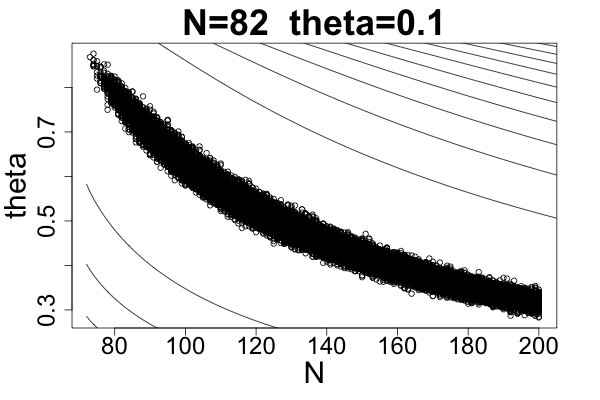
\includegraphics[scale=0.25]{Stat221Waterbuck6.png}
\end{center}
\begin{center}
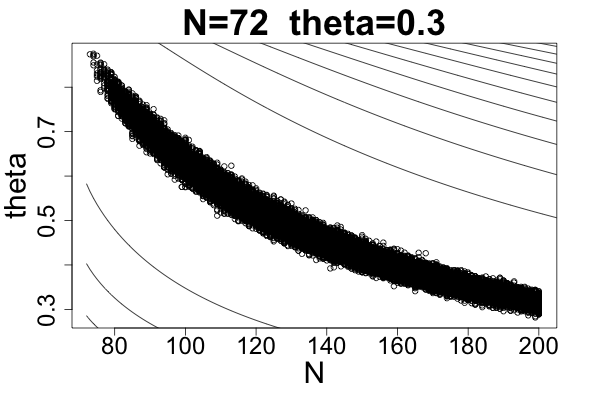
\includegraphics[scale=0.25]{Stat221Waterbuck2.png}
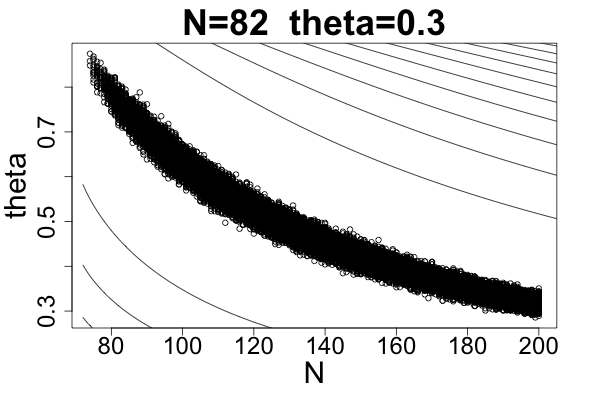
\includegraphics[scale=0.25]{Stat221Waterbuck7.png}
\end{center}
\begin{center}
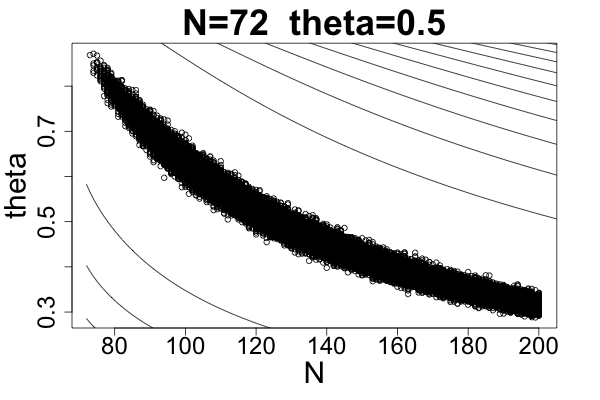
\includegraphics[scale=0.25]{Stat221Waterbuck3.png}
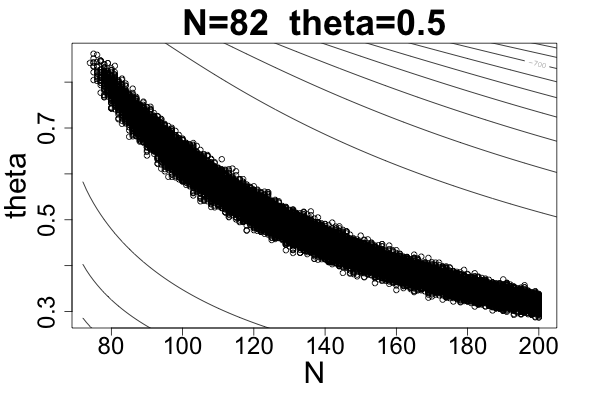
\includegraphics[scale=0.25]{Stat221Waterbuck8.png}
\end{center}
\begin{center}
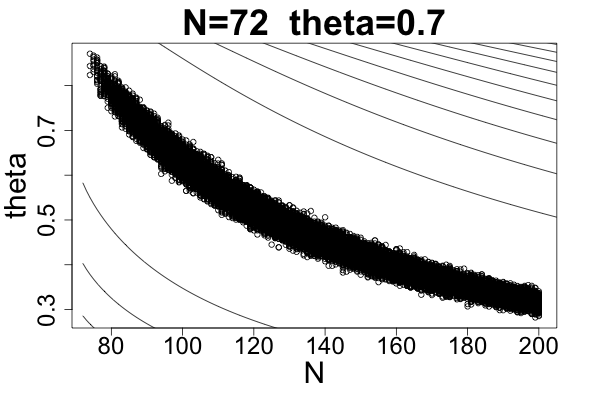
\includegraphics[scale=0.25]{Stat221Waterbuck4.png}
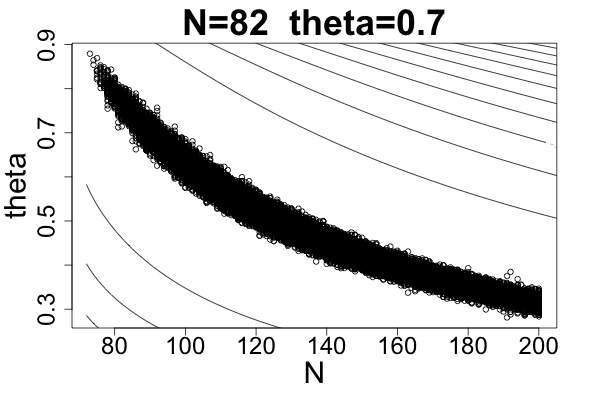
\includegraphics[scale=0.25]{Stat221Waterbuck9.png}
\end{center}
\begin{center}
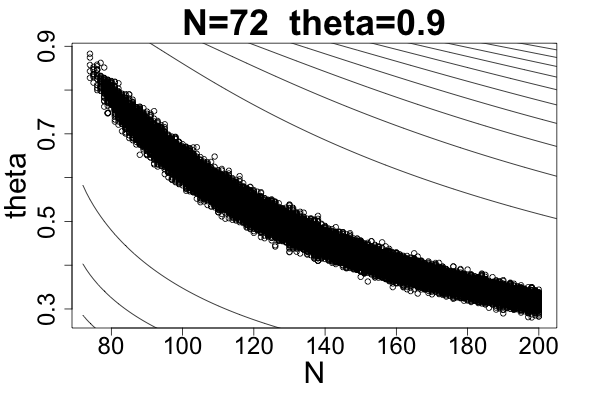
\includegraphics[scale=0.25]{Stat221Waterbuck5.png}
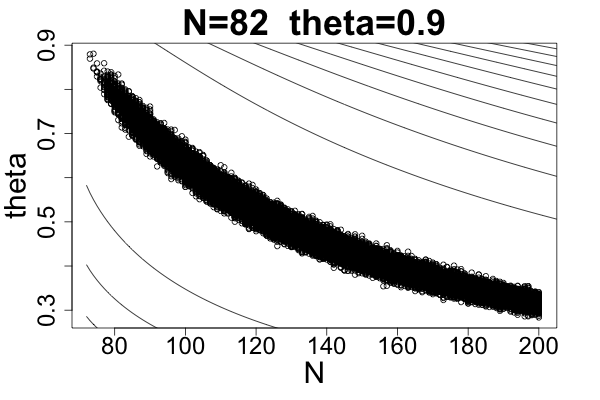
\includegraphics[scale=0.25]{Stat221Waterbuck10.png}
\end{center}
We note that the plots all seem to be very similar, so the starting point is irrelevant to the eventual sample. We include extra diagnostics plot for the last case ($N=82$, $\theta=0.9$) only because there would be too many plots otherwise. We inspect the autocorrelation functions of $N$ and $\theta$ as well as their trace plots. 
\begin{center}
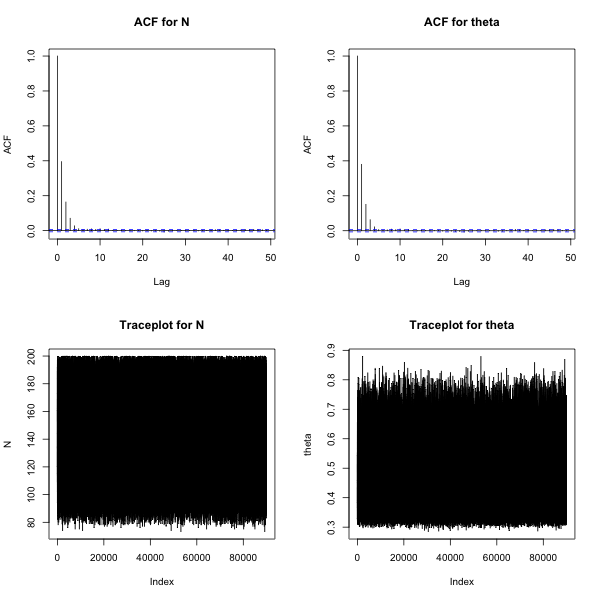
\includegraphics[scale=0.75]{Stat221WaterbuckDiag.png}
\end{center}
We see the ACF plots go to 0 pretty quickly, indicating that there is good mixing. The traceplots cover most of the range of the data, so this is a good sampler.

If we do the same thing with impala, we have
\begin{center}
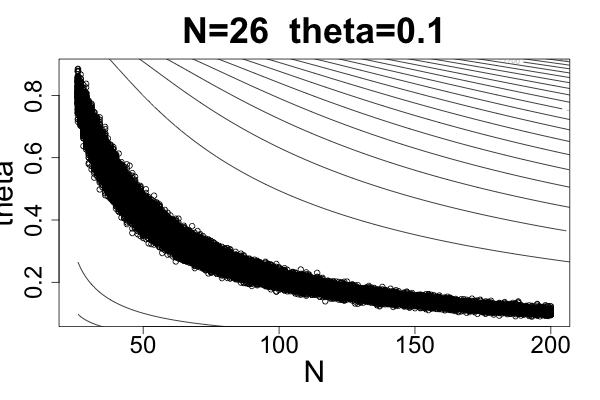
\includegraphics[scale=0.25]{Stat221Impala1.png}
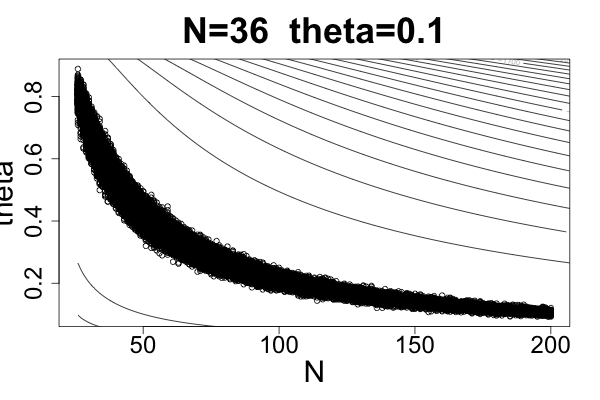
\includegraphics[scale=0.25]{Stat221Impala6.png}
\end{center}
\begin{center}
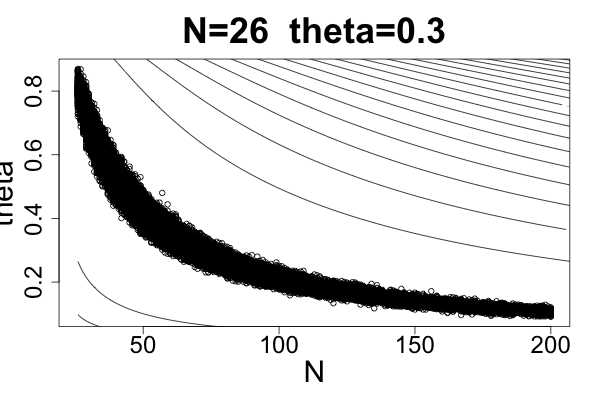
\includegraphics[scale=0.25]{Stat221Impala2.png}
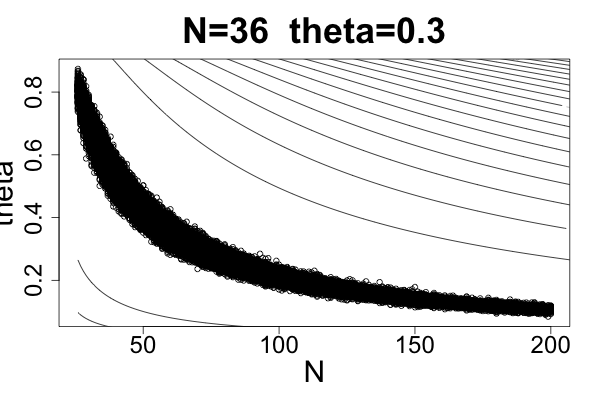
\includegraphics[scale=0.25]{Stat221Impala7.png}
\end{center}
\begin{center}
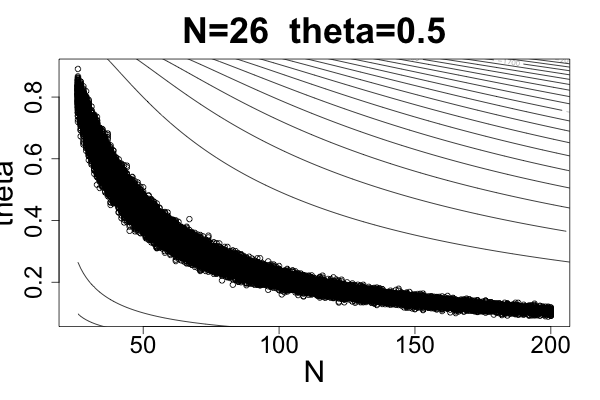
\includegraphics[scale=0.25]{Stat221Impala3.png}
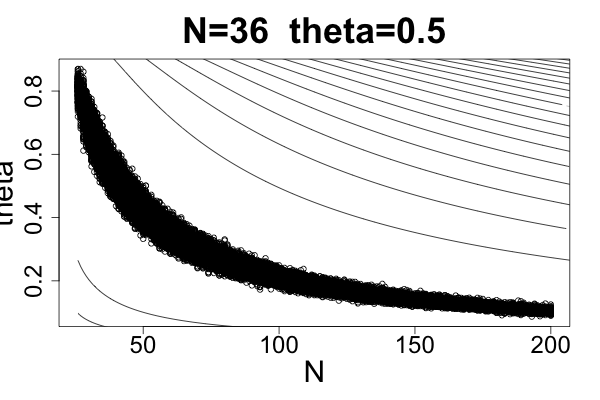
\includegraphics[scale=0.25]{Stat221Impala8.png}
\end{center}
\begin{center}
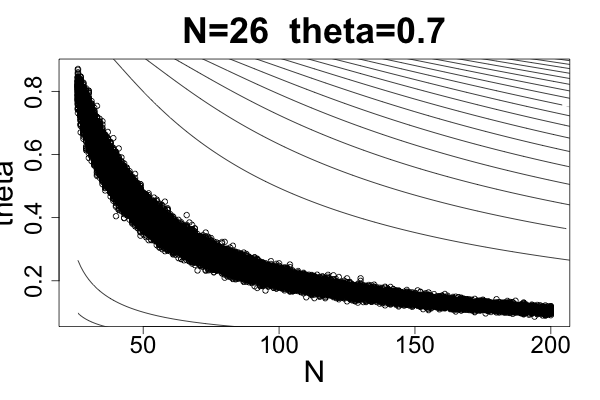
\includegraphics[scale=0.25]{Stat221Impala4.png}
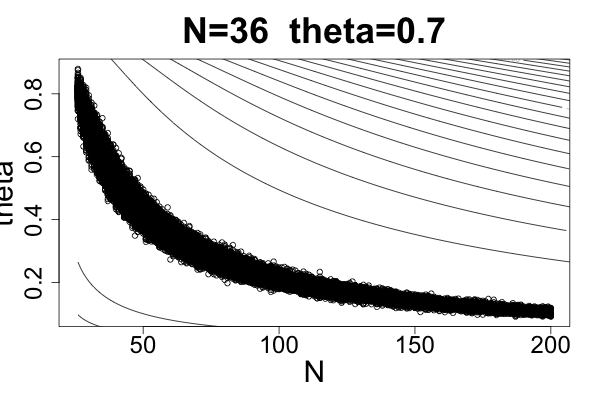
\includegraphics[scale=0.25]{Stat221Impala9.png}
\end{center}
\begin{center}
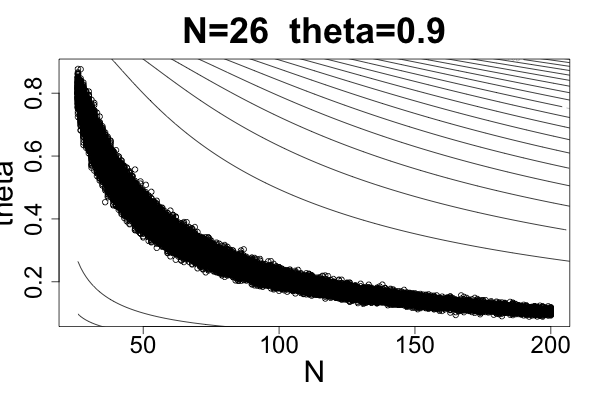
\includegraphics[scale=0.25]{Stat221Impala5.png}
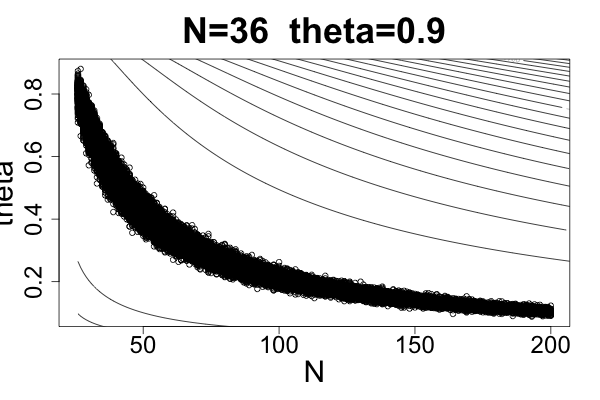
\includegraphics[scale=0.25]{Stat221Impala10.png}
\end{center}
As before, we have that the plots are all very similar, so the starting point for the Metropolis-Hastings algorithm does not have much of an effect. For diagnostics we look at the ACF and trace plots for the last case: 
\begin{center}
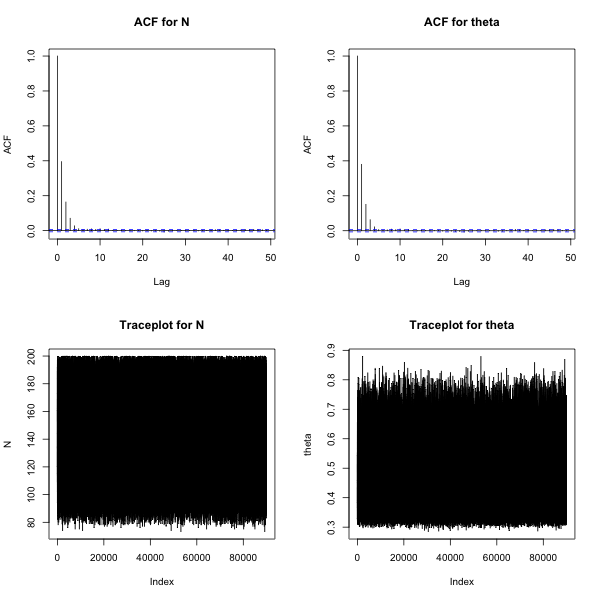
\includegraphics[scale=0.75]{Stat221WaterbuckDiag.png}
\end{center}
We see the same thing as above, so this is a good sampler.


\item
Recall that our posterior density of $(N,\theta)$ was 
\[\p{N, \theta} \propto \left\{\prodin \binom{N}{y_i}\right\}\frac{1}{N} \theta^S (1-\theta)^{nN-S} \mathds{1}_{\theta \in [0,1]}\\ \]
where $S = \sumin y_i$. To find the marginal posterior distribution for $N$, we simply integrate out $\theta$. 
\begin{align*}
\p{N | Y_1, \ldots, Y_n} &= \int_0^1 \! \p{N, \theta | Y_1, \ldots, Y_n} \, \rmd \theta\\
&\propto \int_0^1 \! \theta^S (1-\theta)^{nN - S} \left\{\prodin \binom{N}{y_i}\right\}\frac{1}{N}  \, \rmd \theta\\
&\propto \frac{\Gamma(S+1) \Gamma(nN - S + 1)}{\Gamma(nN+2)}\left\{\prodin \binom{N}{y_i}\right\}\frac{1}{N} \\
&\propto \frac{S!(nN-s)!}{(nN+1)!} \left\{\prodin \binom{N}{y_i}\right\}\frac{1}{N}\\
&\propto \frac{1}{\binom{nN}{S}}\frac{1}{nN+1} \left\{\prodin \binom{N}{y_i}\right\}\frac{1}{N}
\end{align*}
Using this, we sum up the scaled marginal posterior for $N=\max(y), \max(y)+1, \ldots, \max(y)+200$. The number 200 is arbitrary here. We just want to have enough points so that the density becomes small enough. Dividing 1 by this sum gives us the normalizing constant. 
\begin{verbatimcode}
impala = read.table("impala.txt", header = TRUE)
impala = impala[,1]

waterbuck = read.table("waterbuck.txt", header = TRUE)
waterbuck = waterbuck[,1]

unscaled.marg.post.N = function(N,y)
{
  S = sum(y)
  n = length(y)
  1/choose(n*N,S) * 1/(n*N+1) * prod(choose(N,y)/N)
}

y = waterbuck
N.seq = seq(max(y),max(y)+200,1)
marg.post.seq = sapply(N.seq, function(temp) unscaled.marg.post.N(temp,y))
waterbuck.constant = 1/sum(marg.post.seq)

y = impala
N.seq = seq(max(y),max(y)+1000,1)
marg.post.seq = sapply(N.seq, function(temp) unscaled.marg.post.N(temp,y))
impala.constant = 1/sum(marg.post.seq)

> waterbuck.constant
[1] 1.603238e+17
> impala.constant
[1] 2.955879e+13
\end{verbatimcode}
So our normalizing constant for waterbuck is $1.6 \times 10^{17}$ and for the impala is $2.96 \times 10^{13}$.


\item
Now that we have our normalizing constants, we can renormalizing our marginal posterior densities for N. Once we do that, we can simply sum up all the values of the marginal posterior density where $N>100$. 
\begin{verbatimcode}
marg.post.N.waterbuck = function(N,y)
{
  S = sum(y)
  n = length(y)
  val = 1/choose(n*N,S) * 1/(n*N+1) * prod(choose(N,y)/N)*waterbuck.constant
  if(is.na(val))
    return(0)
  val
}
marg.post.N.impala = function(N,y)
{
  S = sum(y)
  n = length(y)
  val = 1/choose(n*N,S) * 1/(n*N+1) * prod(choose(N,y)/N)*impala.constant
  if(is.na(val))
    return(0)
  val
}

y = waterbuck
p.waterbuck = sum(sapply(101:7000,function(i) marg.post.N.waterbuck(i,y)))
p.waterbuck

y = impala
p.impala = sum(sapply(101:7000, function(i) marg.post.N.impala(i,y)))
p.impala
\end{verbatimcode}
This gives
\begin{verbatimcode}
> p.waterbuck
[1] 0.6723058
> p.impala
[1] 0.003140613
\end{verbatimcode}
So that for waterbuck, we have $\p{N >100 | Y_1, \ldots, Y_n} = 0.6723$ and for the impala, we have $\p{N > 100 | Y_1, \ldots, Y_n} = 0.00314$. From our 10 posterior probability estimates, we have
\begin{verbatimcode}
> mean(waterbuck.prob)
[1] 0.8920223
> sd(waterbuck.prob)
[1] 0.001497997
> mean(impala.prob)
[1] 0.1521528
> sd(impala.prob)
[1] 0.002352665
\end{verbatimcode}
Based on this, it looks like our analytical posterior probabilities do not match up with the simulated ones. 


\end{enumerate}
\end{document}

